\chapter{非结构网格双曲守恒律有限体积法}
\label{chap:fvm}

% 这一部分文字主要为了引入本章节的内容, 对该章节做一个整体的把握.

% 1. 从数值求解 PDE 的三大方法出发引入有限体积法. 为什么有限差分,
% 有限体积法, 有限元方法中有限体积法相对来讲要适用一些.

% 有限体积法 (Finite Volume Method, FVM) 数值求解微分方程的主要手段
% 之一. ({\todo}之前在引言里面有没有简单的介绍守恒律?) 从物理学角度
% 的守恒律往往是以宏观尺寸下的积分形式展现, 如经典力学的三大守恒定律
% 都是描述一个宏观控制体上某种物理量总和的变化情况. 而通常意义上的双
% 曲型微分方程是在对控制体取极限之后才得到. 不同于有限差分方法是对变
% 换之后的微分形式进行离散, 有限体积法是将积分形式守恒律直接应用于计
% 算单元上面. 因此在一定程度上有限体积法相比有限差分方法更贴近所离散
% 的物理现象本质. 这一点对于数值模拟线性双曲守恒律计算尤为重要. 这是
% 因为其非线性会导致间断解的产生, 而微分方程却无法描述间断现象. 但是
% 另一方面, 积分形式允许间断解的出现. 这使得有限体积法可以更准确的刻
% 画间断的位置. 另外, 控制体形状的任意性使得有限体积法的框架可以同时
% 应用于结构网格和非结构网格计算.
% % 2. 本章主要设计的内容
% 本章主要介绍经典的非结构网格 MUSCL 类型有限体积方法({\todo}引用
% MUSCL 的经典文献), 以及该技术近些年的最新发展.
% 3. 引入第一章的介绍
非线性双曲守恒律方程理论是应用数学的一个重要研究领域, 有着非常丰富
的理论结果. 有限体积法的发展和分析在很大程度上依赖于这些理论结
果. 下面首先给出双曲守恒律相关数学理论的简要介绍.
% The mathematical theory of nonlinear hyperbolic problems is also
% quite beautiful, and the development and analysis of finite
% volume methods requires a rich interplay between this
% mathematical theory, physical modeling, and numer- ical analysis
% (from Leveque)

\section{双曲守恒律}
\label{sec:hyperbolic-conservation-law}

% 介绍双曲守恒律的理论.
% 参考文献:
% + tengfei 的 thesis, 参考其内容划分, 但是要考虑到避免查重的嫌疑.
% + Toro's Sec 2.4 (主要记号要参考这里)

% 包含的主要部分
% + Sec 2.1.1 双曲守恒律的定义 Jacobian 矩阵, 判别方式
% \subsection{基础理论及间断的产生}
% \label{sec:hyperbolic-cl-def}
\subsection{双曲守恒律的定义及其适定性}
\label{sec:hyperbolic-cl-def}

相对于高维情形, 一维双曲守恒律方程的理论相对比较完善. 另一方面, 数
值格式中的一些重要概念, 如熵条件、数值通量、黎曼问题等也都是以一维
双曲守恒律的理论为基础. 因此这一部分简要介绍一维双曲守恒律的基础理
论,
\begin{definition}
  守恒律是指可以写成下面这种形式的微分方程
  \begin{equation}
    \label{eq:conservation-law}
    {\bf{U}}_{t} + {\bf{F}}({\bf{U}})_{x} = {\bf{0}},
  \end{equation}
  其中
  \begin{equation}
    \label{eq:conserve-variable-and-vector-of-flux}
    {\bf{U}} = \left[
      \begin{array}{c}
        u_{1}\\
        u_{2}\\
        \vdots\\
        u_{m}
      \end{array}
    \right], \quad
    {\bf{F}}({\bf{U}}) = \left[
      \begin{array}{c}
        f_{1}\\
        f_{2}\\
        \vdots\\
        f_{m}
      \end{array}
    \right].
  \end{equation}
  称 ${\bf{U}}$ 为守恒变量, ${\bf{F}}({\bf{U}})$ 称为通量.
\end{definition}
注意到 ${\bf{F}} = {\bf{F}}({\bf{U}})$ 是关于 ${\bf{U}}$ 的向量
函数. 可以写出其雅可比矩阵 (Jacobian Matrix)
\begin{equation}
  \label{eq:jacobian-matrix-flux}
  {\bf{A}}({\bf{U}}) =
  {\partial {\bf{F}}}/{\partial {\bf{U}}} = \left[
    \begin{array}{ccc}
      \partial f_{1} / \partial u_{1} &\cdots & \partial f_{1}
      / \partial u_{m}\\
      \partial f_{2} / \partial u_{1} &\cdots & \partial f_{2}
      / \partial u_{m}\\
      \vdots & \ddots & \vdots\\
      \partial f_{m} / u_{1} & \cdots & \partial f_{m} / u_{m}
    \end{array}
  \right].
\end{equation}
对 (\ref{eq:conservation-law}) 式第二项应用链式法则得到守恒律的拟线性形式,
\begin{equation}
  \label{eq:quasi-linear-form-conservation-law}
  {\bf{U}}_{t} + {\bf{A}}({\bf{U}}){\bf{U}}_{x} = 0,
\end{equation}
\begin{definition}
  当守恒律 (\ref{eq:conservation-law}) 通量项的雅可比矩
  阵 (\ref{eq:jacobian-matrix-flux}) 有 $m$ 个实特征根
  $\lambda_{i}({\bf{U}})$ 并且对应的存在一组线性无关的特征向量
  ${\bf{K}}^{(i)}({\bf{U}}), i = 1, \ldots, m$ 时, 称守恒律方程
  (\ref{eq:conservation-law}) 为 {\it 双曲型}. 当 $m$ 个实特征跟
  互不相同时, 则称 (\ref{eq:conservation-law}) 为 {\it 严格双曲型}.
\end{definition}
% + Sec 2.1.2 间断的产生 双曲方程解的适定性问题. 熵 熵条件, 引入
% 熵条件的物理背景. (将这一部分并如基础理论这一部分)
即便初值是光滑的, 随时间演化也会出现间断, 这是非线性双曲型方程的主
要特点之一.  Burgers 方程是最简单的标量非线性双曲方程的例
子, 也称Hopf 方程.
\begin{equation}
  \label{eq:burger-equation}
  u_{t} + {\left( {u^{2}}/{2} \right)}_{x} = 0,
\end{equation}
考虑如下初值问题
\begin{equation}
  \label{eq:burger-equation-initial}
  u(x,0) = u_{0} = \left\{
    \begin{aligned}
      &1 + ({2}/{\pi}) \sin \left( 2x - {\pi}/{2} \right),&
      \quad & \mbox{if}~ x \in [0, \pi]\\
      &1 - {2}/{\pi}, &\quad & \mbox{otherwise}
    \end{aligned}
  \right.
\end{equation}
其精确解随时间变化如
图 (\ref{fig:burgers-shock-formation}) 所示. 注意到在时间推进
到 $T = 0.5 \pi$ 附近精确解出现间断. 事实上, 如果初值$u_{0}$ 是光
滑的并且 $u'_{0}(x)$ 在某处存在负值, 则在
\begin{equation}
  \label{eq:burgers-shock-time}
  T_{b} = \frac{-1}{\min u'_{0}(x)} .
\end{equation}
时一定会形成激波 \cite{LeVeque1992a}.
\begin{figure}[htbp]
  \centering
  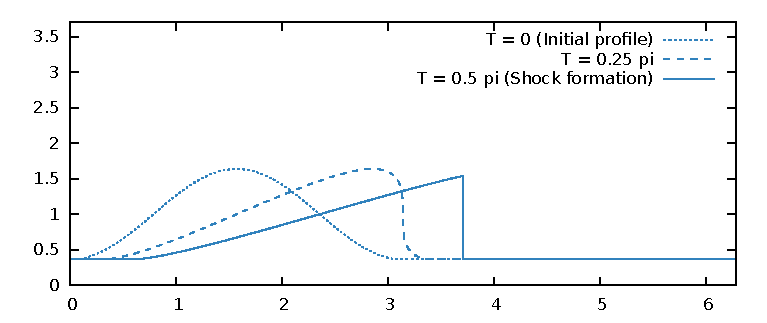
\includegraphics[width=1.0\linewidth]{./Pho/Chp2/exact_burgers.pdf}
  \caption{Burgers 方程间断解形成过程}
  \label{fig:burgers-shock-formation}
\end{figure}

% to be continue
由于间断处的导数不存在, 所以间断解不是传统意义上的解, 无法用传统的
微分方程进行描述. 为此需要引入弱解的概念, 通过在广义的意义上满足微
分方程的方式刻画间断解这一类更广泛的解. 下面为叙述方便考虑一般形式
的标量双曲守恒律,
\begin{equation}
  \label{eq:scaler-hyperbolic-conservation-law}
  u_{t} + f(u)_{x} = 0,
\end{equation}
% Def 弱解
方程 (\ref{eq:scaler-hyperbolic-conservation-law}) 的弱解定义如下,
\begin{definition}
  如果函数 $u(x,t)$ 满足, 对于任意的 {\it 测试函数} $\phi \in
  C_{0}^{1}$ 都成立
  \begin{equation}
    \label{eq:conservation-law-weak-form}
    \int_{0}^{\infty} \int_{-\infty}^{+\infty} \left( \phi_{t}u +
      \phi_{x}f(u)\right) \dd x \dd t = - \int_{-\infty}^{+\infty}
    \phi (x,0) u(x,0) \dd x,
  \end{equation}
  则称 $u(x,t)$ 为方
  程(\ref{eq:scaler-hyperbolic-conservation-law}) 的{\it 弱解}.
\end{definition}
满足 (\ref{eq:conservation-law-weak-form}) 的解不是唯一的. 但是在
实际问题中通常以粘性项趋向于零时解的极限状态作为物理可允许解. 因此
需要引入 {\it 熵条件} 的概念对满足
条件的弱解进行筛选. 熵条件对应了热力学第二定律(熵增定律). 在空气动
力学中, {\it 熵}在连续流场的路径上保持不变, 跨过激波时值变大, 不会
出现值变小的情况. 针对实际的需要可以设计出不同形式的熵条件, 通过推
广物理上熵的概念定义熵函数、熵通量及熵不等式的方式给出熵条件是其中
一种重要的形式. 关于熵条件的详细介绍可以参
考 Chorin、Marsden\cite{Chorin1993} 和 LeVeque
\cite{LeVeque1992a}. 另外, 熵条件在离散情形下的推广在数值格式的设
计和分析中有着重要的应
用 \cite{Majda1979,Osher1984,Jiang1994,Hou2006}. 例如, 如果数值格
式满足离散的熵不等式, 则可以确保数值解收敛得到物理可允许解, 这对
于检验数值方法的正确性有着重要的意义.

% TODO 解的适定性问题?
一般形式的双曲守恒律方程的适定性问题是应用数学领域重要的开放性问题
之一.  在一维情形则有相对丰富的理论支持, 但是针对高维情形的理论建
立非常困难. Lax 于 1957 年 \cite{Lax1957} 解决了一维双曲守恒律方程
组 Riemann 问题的适定性问题. 对于一般的初值问题,
Glimm 于1965 年 \cite{Glimm1965} 引入随机选择法 (Random Choice
Method) 成功解决了其解的存在性问题. 但是该方法只适用于每个特征向量
场要么是本质非退化要么是线性退化的守恒律方程, 这种类型的方程的典型
例子就是气体动力学中的 Euler 方程. 对于一般情形建立完整的适定性理
论仍然十分困难. 双曲守恒律整体解的理论研究在上世纪后半叶一直是一个
比较活跃的研究领域 . 直到 Liu、Yang 在 1999 年\cite{Liu1999} 引入
广义熵泛函 --- ``Liu-Yang 泛函'' 才对一维双曲守恒律方程组建立起一
个圆满的适定性理论.

% 熵条件可以视为热力学第二定律的一个推广 这些熵条件里面最主要的一种
% 表述方式为 熵不等式的形式进行表述. 这对于数值方法也有着同样重要的
% 意义, (为了确保数值上得到的解是对物理可允许解的一个正确的近似)因此
% 有对应的离散熵条件. 双曲守恒律解的适定性问题仍然是一个开放性问题.
% ({\todo} verify this statement)

% + Sec 2.1.3 例子 可以最后讲到欧拉方程的时候简要介绍一下 Riemann
% 问题, 指向参考文献就可以了.
\subsection{实例}
\label{sec:hyperbolic-conservation-law-examples}
许多实际应用的数学模型可以归结到双曲守恒律. 这一部分介绍几个重要
的双曲守恒律的例子.

\begin{example}
  首先介绍两个常见的多维标量双曲方程的例子. 考虑如下形式的标量守
  恒律方程,
  \begin{equation}
    \label{eq:multi-dim-scaler-equation}
    u_{t} + {\bf{a}} \cdot \nabla u = 0.
  \end{equation}

  如果将 (\ref{eq:multi-dim-scaler-equation}) 式中的系
  数${\bf{a}}$ 取为固定值, 则方程称为 {\it 线性对流方程}, 是为最简
  单的双曲守恒律方程. 描述了初始数据整体以速度 ${\bf{a}}$传播的过
  程. 配合周期边界条件, 常用于测试计算格式的准确性和数值精度.

  若令 ${\bf{a}} = \left( -(y-c_{x}), (x-c_{y})
  \right)$ 则 (\ref{eq:multi-dim-scaler-equation}) 称为旋转对流问
  题. 用于描述以恒定角速度 $2\pi$ 绕中心点 $(c_{x}, c_{y})$ 旋转的
  图像. 由于容易获得精确解, 该算例也常用于检验算法的正确性和数值精
  度.

\end{example}
\begin{example}
  欧拉方程是应用最广泛的双曲守恒律模型, 这里我们仅以一维情形为例,
  高维欧拉方程的介绍参考 Toro \cite{Toro2009} 第三章的内容. 一维
  其表述如下,
  \begin{equation}
    \label{eq:1d-euler-eq}
    \begin{aligned}
      &{\bf{U}}_{t} + {\bf{F}}({\bf{U}})_{x} = 0,\\
      &{\bf{U}} = \left[
        \begin{array}{c}
          \rho\\
          \rho u\\
          E
        \end{array}
      \right], \quad
      {\bf{F}}({\bf{U}})\left[
        \begin{array}{c}
          \rho u\\
          \rho u^{2} + p\\
          u(E + p)
        \end{array}
      \right].
    \end{aligned}
  \end{equation}
  其中三个偏微分方程分别对应于质量守恒、动量守恒和能量守恒. 其中
  \begin{equation}
    \label{eq:energy-euler}
    E = \rho \left( e + \frac{1}{2} u^{2} \right)
  \end{equation}
  为动能和内能之和. 方程组 (\ref{eq:1d-euler-eq})本身不是封闭的,
  另外缺少如下的理想气体状态方程,
  \begin{equation}
    \label{eq:idea-gas}
    e = \frac{p}{\rho (\gamma - 1)}.
  \end{equation}
  其中, $\gamma$ 为常数, 对于空气应取 $\gamma = 1.4$.
\end{example}
\begin{example}
  二维浅水波方程,
  \begin{equation}
    \label{eq:shallow-water-equation}
    \begin{aligned}
      h_{t} + (hu)_{x} + (hv)_{y} = 0,\\
      (hu)_{t}+ \left( hu^{2} + \frac{1}{2}gh^{2} \right)_{x} +
      (huv)_{y} = 0,\\
      (hv)_{t} + (huv)_{x} + \left( hv^{2} + \frac{1}{2}
        gh^{2}\right)_{y} = 0,
    \end{aligned}
  \end{equation}
  其中 $h$ 表示深度, $(u,v)$ 为速度向量, 那么 $hu, hv$ 分别表征了
  两个方向上的动量.
\end{example}

% \section{非结构网格生成技术}
% \label{sec:unstru-mesh-technique}
% 这一部分包含下面几个方面的内容
% 1. 两种主流的非结构网格生成方法
% 2. 对网格进行 smooth 的常用方法.
% 3. 如何判断网格的好坏.
% 4. 非结构网格生成工具 GMSH 的简单介绍 (主要提一下)

\section{有限体积法}
\label{sec:fvm-discrect}
\subsection{空间离散}
\label{sec:semi-descrete-form}
在这一部分我们考虑高维守恒律方程组,
\begin{equation}
  \label{eq:multi-dim-conservation-law}
  {\bf{U}}_{t} + \nabla \cdot {\bf{F}}({\bf{U}}) = 0,
\end{equation}
首先考虑如何进行空间离散. 设 $\Omega \in \RealR^{d}$ 为计算区
域. 其上的网格单元剖分 $\mathcal{T} = \left\{ T_{k} \right\}$ 满
足条件
\begin{equation}
  \label{eq:region-decomposition}
  \begin{aligned}
    &\bigcup_{T_{k}\in \mathcal{T}} {T}_{k} = {\Omega},\\
    &T_{k} \bigcap T_{l} = \varnothing, \quad \forall T_{k},T_{l} \in \mathcal{T}.
  \end{aligned}
\end{equation}
记守恒量的单元平均值
\begin{equation}
  \label{eq:average-fvm}
  \bar{{\bf{U}}}_{j} = \frac{1}{\vert T_{j} \vert} \int_{T_{j}}
  {\bf{U}} \dd x.
\end{equation}
将守恒律方程 (\ref{eq:multi-dim-conservation-law}) 在 $T_{j}$ 上积
分, 再对第二项利用 Green 公式, 得到守恒律的积分形式如下,
\begin{equation}
  \label{eq:conservation-law-integral-form}
  \left( \bar{{\bf{U}}}_{j} \right)_{t} + \frac{1}{\vert T_{j} \vert} \oint_{\partial T_{j}}
  {\bf{F}}({\bf{U}}) \cdot {\bf{n}}~ \dd \Gamma = 0,
\end{equation}
其中 ${\bf{n}}$ 为边界上的外法向.
% 通常情况下单元边界可以分解为几个
% 互不重叠且形式相对简单的边并, 即存在 $\left\{ e_{i}^{(k)}
% \right\}, e_{i}^{(k)} \in $
% \begin{equation}
%   \label{eq:union-of-element-boundary}
%   \begin{aligned}
%     &\partial T_{k}  = \bigcup_{i = 1}^{n_{k}} e_{i}^{(k)},\\
%     &e_{i}^{(k)} \bigcap e_{j}^{(k)} = \varnothing, \quad \forall
%     i\neq j,
%   \end{aligned}
% \end{equation}
% 其中 $n_{k}$ 为 $T_{k}$ 的边界个数.
将单元边界拆分成几个互不重合的面, 可以
将 (\ref{eq:conservation-law-integral-form}) 式进一步写成下面的形
式,
\begin{equation}
  \label{eq:conservation-law-integral-form-2}
  \left( \bar{{\bf{U}}}_{j} \right)_{t} + \frac{1}{\vert T_{j} \vert}
  \sum_{e \in \partial T_{j}}\int_{e}{\bf{F}}({\bf{U}}) \cdot
  {\bf{n}}_{e, T_{j}} \dd \Gamma = 0,
\end{equation}
处理(\ref{eq:conservation-law-integral-form-2}) 的第二项需要引入数
值通量和数值积分两种技术手段.

数值通量的引入则是为了处理跨过单元边界两侧解的不连续问题. 注意到有
限体积离散解 ${\bf{U}}$ 在边界面 $e$ 两侧有不同的重构值, 因此第二
项积分项 ${\bf{F}}({\bf{U}}) \cdot {\bf{n}}_{e,T_{j}}$ 没有确
切的定义. 为此, 引入 {\it 数值通量} ${\bf{h}}_{e, T_{j}}
({\bf{U}}^{int}_{j}(t, x)), {\bf{U}}^{ext}_{j}(t, x),
{\bf{n}}_{e, T_{j}})$. 其中${\bf{U}}_{j}^{int/ext} (t,x)$ 分别
为单元边界 $e$ 上 $x$ 处的内外侧重构值. 通常来说数值通量函
数 ${\bf{h}}_{e,T}$ 应是局部 Lipschitz 连续的, 并且需要满足下面两
个条件,
\begin{equation}
  \label{eq:numerical-flux-condition}
  \begin{aligned}
    & {\bf{h}}_{e,T}({\bf{U}},{\bf{U}},{\bf{n}}) =
    {\bf{F}}({\bf{U}}) \cdot {\bf{n}},  &
    \quad & \mbox{(相容性)}\\
    & {\bf{h}}_{e,T}({\bf{U}}^{int},{\bf{U}}^{ext},{\bf{n}}) =
    -{\bf{h}}_{e,T'_{e}}({\bf{U}}^{ext},{\bf{U}}^{int},-{\bf{n}}) &
    \quad & \mbox{(守恒性)}
  \end{aligned}
\end{equation}
其中 $T'_{e}$ 表示 $T$ 在边 $e$ 一侧的邻居单元.

数值积分是将连续的积分在保持必要的精度的前提下近似转化为可计算的离散形
式. 数值积分可以
以如下方式表述,
\begin{equation}
  \label{eq:numerical-integral}
  \int_{e} {\bf{h}}_{e,T} (t,x) \dd \Gamma \approx
  \sum_{l=1}^{L} \omega_{l} {\bf{h}}_{e,T}(t,x_{e,l}) \vert e \vert,
\end{equation}
其中积分点 $x_{e,l}$ 及系数 $\omega_{l}$ 的确定与具体的数值积分方
法有关. 一维数值积分理论可以参考文
献 \cite{LiBook1978}. 文献 \cite{zhang2009set} 则对三角形单元及四
面体单元的数值积分做了详尽的分析. 将数值积分和数值通量技术应用
到 (\ref{eq:conservation-law-integral-form-2}) 式, 对第二项进行进
一步转化, 得到如下半离散形式
\begin{equation}
  \label{eq:semi-discrect-method}
  \left( \bar{{\bf{U}}}_{j} \right)_{t} = - \frac{1}{\vert T_{j} \vert}
  \sum_{e \in \partial T_{j}}\sum_{l=1}^{L} \omega_{l}
  {\bf{h}}_{e,T_{j}}({\bf{U}}_{j}^{int}(t,x_{e,l}),
  {\bf{U}}_{j}^{ext}(t, x_{e,l}), {\bf{n}}_{e,T_{j}}) \vert e \vert
\end{equation}

在这篇文章中我们主要介绍下面两种数值通量函数,
\begin{itemize}
\item Local Lax-Friedrichs (LLF) 通量,
  \begin{equation}
    \label{eq:local-lax-friedrichs-flux}
    {\bf{h}}({\bf{U}},{\bf{V}},{\bf{n}}) = \frac{1}{2}
    \left(
      {\bf{F}}({\bf{U}}) \cdot {\bf{n}} + {\bf{F}}({\bf{V}})
      \cdot {\bf{n}} - \alpha_{e,k} \left( {\bf{V}} - {\bf{U}} \right)
    \right).
  \end{equation}
  其中 $\alpha_{e,j}$ 是单元 $T_{j}$ 上 Jacobian 矩阵 $\frac{\partial}{\partial
    {\bf{U}}} \left( {\bf{F}}\left( \bar{{\bf{U}}}_{j}
    \right)\cdot {\bf{n}}_{e,T_{j}} \right)$ 的绝对值最大的特征值.
  LLF 通量会引入较大的数值耗散, 对间断的分辨率比较差. 但是 LLF通
  量计算时间较少, 且相对来讲有更好的稳定性.
\item HLLC 通量是 Toro、Spruce 等学者对 HLL 通量的改进, 将求解区域
  按照左右两个非线性波及中间的接触间断分为四个常数区域, 克服
  了 HLL 通量无法处理接触间断和剪切波的问题, 详细说明参考文
  献 \cite{Toro1994,Harten1983b}. HLLC 通量本质上是在边界积分点处以
  两侧守恒量的重构值为左右两个状态求解近似 Riemann 问题, 得到一个
  交界面处的近似值 ${\bf{U}}^{*}\left( {\bf{U}}^{int},
    {\bf{U}}^{ext},{\bf{n}} \right)$, 从而得到对通量的一个合理的近
  似 ${\bf{F}}({\bf{U}}^{*})\cdot {\bf{n}}$. 这是数值通量的主要
  处理方式之一,其核心是如何构造合理的近似 Riemann 求解
  器, 文献 \cite{Toro2009} 给出了多种类型的 Riemann 求解器的详细分
  析.

  下面考虑 Euler 方程 x-split 三维 Riemann 问题,
  \begin{equation}
    \label{eq:x-split-3d-Riemann}
    \begin{aligned}
      &{\bf{U}}_{t}+{\bf{F}}({\bf{U}})_{x} = 0,\\
      &{\bf{U}}(x,0) = {\bf{U}}^{(0)} = \left\{
        \begin{aligned}
          &{\bf{U}}_{L} \quad & x < 0,\\
          &{\bf{U}}_{R} \quad & x > 0.
        \end{aligned}
      \right.
    \end{aligned}
  \end{equation}
  其中,
  \begin{equation}
    \label{eq:x-split-3d-Riemann-variable-and-flux}
    {\bf{U}} = \left[
      \begin{array}{c}
        \rho\\
        \rho u\\
        \rho v\\
        \rho w\\
        E
      \end{array}
    \right], \quad {\bf{F}}({\bf{U}}) = \left[
      \begin{array}{c}
        \rho u\\
        \rho u^{2} + p\\
        \rho u v\\
        \rho u w\\
        u (E + p)
      \end{array}
    \right].
  \end{equation}

  HLLC 通量的计算可以大致分为如下三个步骤,
  \begin{itemize}
  \item[Step 1] 为了给出波速 $S_{L},S_{R},S_{*}$ 的估计, 首先需要
    近似计算两侧线性波之间的区域压强. Toro 将这一区域称为 {\it
      Star Region}. 下面对压强的估计方法来源于 PVRS 近似 Riemann
    求解器, 是一种线性近似方法,
    \begin{equation}
      \label{eq:pre-est}
      p_{\ast} = \max \left( 0, p_{\mbox{\scriptsize pvrs}}
      \right),
    \end{equation}
    % 其中 $p_{\mbox{\scriptsize pvrs}}$ 是一种估计中压强的方法.
    \begin{equation}
      \label{eq:star-p}
      p_{\mbox{\scriptsize pvrs}} = \frac{1}{2}(p_{L} + p_{R}) -
      \frac{1}{2}(u_{R} - u_{L}) \bar{\rho} \bar{a},
    \end{equation}
    其中,
    \begin{equation}
      \label{eq:average-rho-sonic}
      \bar{\rho} = \frac{1}{2} (\rho_{L} + \rho_{R}), \quad
      \bar{a} = \frac{1}{2} (a_{L} + a_{R}).
    \end{equation}
  \item[Step 2] 估计波速. 首先估计左右两个非线性波的波速 $S_{L}, S_{R}$,
    \begin{equation}
      \label{eq:wave-speed}
      S_{L} = u_{L} - a_{L}q_{L}, \quad S_{R} = u_{R} + a_{R} q_{R}
    \end{equation}
    其中,
    \begin{equation}
      \label{eq:q-symbol}
      q_{K} = \left\{
        \begin{aligned}
          & 1 & ~\mbox{\scriptsize if} ~ p_{\ast} \le p_{K}\\
          &\left[ 1 + \frac{\gamma + 1}{2\gamma} \left(
              \frac{p_{\ast}}{p_{K}} - 1 \right)
          \right]^{\frac{1}{2}} & ~\mbox{\scriptsize if} ~
          p_{\ast} > p_{K}.
        \end{aligned}
      \right.
    \end{equation}
    其中 $K=L$ 或 $K=R$ 对应了左右两侧的状态. 用这些估计值继续估
    计 Star Region 里面接触间断的波速,
    \begin{equation}
      \label{eq:star-region-estimate-sonice-speed}
      S_{\ast} = \frac{p_{R} - p_{L} + \rho_{L} u_{L}(S_{L} -
        u_{L}) -
        \rho_{R}u_{R}(S_{R}-u_{R})}{\rho_{L}(S_{L}-u_{L}) -
        \rho_{R}(S_{R}- u_{R})}.
    \end{equation}
    这里 $S_{L}, S_{R}$ 的计算方式还有很多其他的选择, 参考 \cite{Toro2009}.
  \item[Step 3] 计算 HLLC 通量.
    \begin{equation}
      \label{eq:HLLC-flux}
      {\bf{F}}_{i+\frac{1}{2}}^{\mbox{\scriptsize hllc}} =
      \left\{
        \begin{aligned}
          {\bf{F}}_{L} & ~\mbox{\scriptsize if} \quad & 0 \le
          S_{L},\\
          {\bf{F}}_{\ast L} & ~\mbox{\scriptsize if} \quad &
          S_{L} \le 0 \le S_{\ast},\\
          {\bf{F}}_{\ast R} & ~\mbox{\scriptsize if} \quad &
          S_{\ast} \le 0 \le S_{R},\\
          {\bf{F}}_{R} & ~\mbox{\scriptsize if} \quad & 0 \ge S_{R},
        \end{aligned}
      \right.
    \end{equation}
    其中
    \begin{equation}
      \label{eq:star-region-flux}
      {\bf{F}}_{\ast K} = {\bf{F}}_{K} + S_{K}({\bf{U}}_{\ast K}
      - {\bf{U}}_{K})
    \end{equation}
    \begin{equation}
      \label{eq:star-region-value}
      {\bf{U}}_{\ast K} = \rho_{K} \left(
        \frac{S_{K}-u_{K}}{S_{K}-S_{\ast}}
      \right)
      \left[
        \begin{array}{c}
          1\\
          S_{\ast}\\
          v_{K}\\
          w_{K}\\
          \frac{E_{K}}{\rho_{K}} + (S_{\ast}-u_{K})
          \left[
            S_{\ast} + \frac{p_{K}}{\rho_{K}(S_{K}-u_{K})}
          \right].
        \end{array}
      \right]
    \end{equation}
  \end{itemize}
\end{itemize}
% 注意到上面给出的计算是针对 x-split 3D Riemann 问题. 是否应该给出
% 一般方向上的 HLLC 通量表述.

% \subsection{重构过程及 MUSCL 类型方法}
% \label{sec:muscl-type-method}
\subsection{离散精度及重构过程}
\label{sec:accuracy-and-reconstruction}


% 1. 介绍重构之前可以先讲一下半离散格式的精度问题. 即重构阶数如何影
% 响数值解的精度阶数.
在介绍重构过程之前, 首先引入空间离散精度的概念. 综合所有单元,
半离散方程 (\ref{eq:semi-discrect-method}) 式事实上是一个守恒量单元平均值关于
时间 $t$ 的常微分方程组, 可以记为
\begin{equation}
  \label{eq:semi-descrect-ode}
  \bar{{\bf{U}}}'(t) = \mathcal{L} \left( \bar{{\bf{U}}}(t) \right),
\end{equation}
其中 $\bar{{\bf{U}}}(t)$ 是分片常值函数, 例如其在单元 $T_{j}$ 上的
值为 $\bar{{\bf{U}}}_{j}$. $\mathcal{L}$ 是空间离散算子. 注意
到 (\ref{eq:semi-descrect-ode}) 式其实是守恒律的积分形
式 (\ref{eq:conservation-law-integral-form-2}) 在引入数值通量及数
值积分之后的近似处理. 下面记在单元 $T_{j}$ 上精确解的单元平均值
为 $\bar{\bf{u}}_{j}(t)$. 若
\begin{equation}
  \label{eq:spatial-accuracy}
  \bar{{\bf{U}}}_{j}(t) = \bar{{\bf{u}}}_{j}(t) +
  \mathcal{O}(D(T_{j})^{p}), \quad \vert T_{j} \vert \rightarrow 0.
\end{equation}
则称半离散形式 (\ref{eq:semi-descrect-ode}) 有 $p$ 阶的空间离散精
度.

注意到对于有限体积法来说, 所有的计算都是对单元平均值进行的. 当计算
进行到某一时间步时, 计算下一时间层的数值信息就只有上一层单元平均
值. 因此问题的关键就是如何通过网格平均值 $\bar{\bf{U}}_{j}$ 及几何
信息得到 Gauss 点处对函数值 ${\bf{u}}_{j}$ 的高精度近似. 这一过程
称为重构. 寻找有效的重构方法近些年来有限体积法领域的热点研究问题.
van Leer \cite{VANLEER1974361,Leer1979} 利用相邻单元的信息进行线性
重构, 并引入斜率限制器以抑制数值震荡的产生. 这种重构策略称
为 MUSCL 重构. 基于这一重构策略的数值方法在之后得到了广泛的发展,
Osher \cite{Osher1985} 对半离散形式的一维 MUSCL 方法进行了详细的分
析.  MUSCL 格式由于其健壮性而被广泛应用于实际的工程计算
中. 基于 MUSCL 重构的思想依次出现了 PPM
\cite{Colella1984}、ENO/WENO \cite{Shu1988,Liu1994} 等高阶重构方
法. 但是相比 MUSCL 重构, 这些高阶方法很难推广到非结构网格. 本文主
要讨论非结构网格上的 MUSCL 类型重构方法.

对于计算格式, 我们总希望获得更高的数值精度. 半离散方法将空间离散和
时间离散进行分离, 从而非常适合高精度格式的构造. 其中空间离散精度的
阶数取决于数值积分的精度以及数值通量对真实通量的近似阶数. 我们
在 (\ref{sec:semi-descrete-form}) 一节中讨论了两种数值通量的构造方
法, 其计算皆依赖于两侧的重构值 ${\bf{U}}^{int/ext}$. 事实上只要数
值通量满足基本的条件 (\ref{eq:numerical-flux-condition}), 对原通量
的逼近精度就完全取决于重构值的精度. 因此重构精度是获得高精度空间的
离散的主要因素, 相关的可以理论参考文献 \cite{LeVeque1992a} 第十七
章.

\subsection{时间离散}
\label{sec:time-stepping-methods}

要进行完整的有限体积法求解还需要在时间方向上离散常微分方程
组(\ref{eq:semi-descrect-ode}). 在之前的部分我们讨论了空间离散的重
要性, 但是要使得数值解达到期望的精度还需要采用高阶的时间离散方
法. 本文采用 Shu 、Osher \cite{Shu1988} 提出的一类具有 SSP
(Strong Stability Preserving) 性质的高阶 Runge-Kutta 方法. 在具体
计算中常用的是如下``最优的'' 二阶与三阶方法.

\begin{itemize}
\item 二阶方法
  \begin{equation}
    \label{eq:second-order-rk}
    \begin{aligned}
      &\tilde{{\bf{U}}}^{(0)} & := &{\bf{U}}^{n},\\
      &\tilde{{\bf{U}}}^{(1)} & := &{\bf{U}}^{(0)} + \Delta t ~
      \mathcal{L} \left( \tilde{{\bf{U}}}^{(0)} \right),\\
      &{\bf{U}}^{n+1} & := &\frac{1}{2}\tilde{\bf{U}}^{(0)} +
      \frac{1}{2}\tilde{{\bf{U}}}^{(1)} + \frac{1}{2} \Delta t ~
      \mathcal{L} \left( \tilde{{\bf{U}}}^{(1)} \right).
    \end{aligned}
  \end{equation}
\item 三阶方法
  \begin{equation}
    \label{eq:3rd-rk}
    \begin{aligned}
      & \tilde{{\bf{U}}}^{(0)} & := & {\bf{U}}^{n},\\
      & \tilde{{\bf{U}}}^{(1)} & := & \tilde{{\bf{U}}}^{(0)} +
      \Delta t ~ \mathcal{L} \left( \tilde{{\bf{U}}}^{(0)}
      \right),\\
      & \tilde{{\bf{U}}}^{(2)} & := &
      \frac{3}{4}\tilde{{\bf{U}}}^{(0)} +
      \frac{1}{4}\tilde{{\bf{U}}}^{(1)} + \frac{1}{4} \Delta t ~
      \mathcal{L} \left( \tilde{{\bf{U}}}^{(1)} \right),\\
      & {\bf{U}}^{n+1} & := & \frac{1}{3} \tilde {{\bf{U}}}^{(0)}
      + \frac{2}{3} \tilde{{\bf{U}}}^{(2)} + \frac{2}{3} \Delta t
      ~ \mathcal{L} \left( \tilde{{\bf{U}}}^{(2)} \right).
    \end{aligned}
  \end{equation}
\end{itemize}

\subsection{非结构网格 MUSCL 类型重构}
\label{sec:MUSCL-on-unstru}
按照数据存储依附的位置不同, 有限体积法分为格子中心方
法 (cell-centered method) 和节点中心方法 (vertex-based method 或
cell-vertex method). 前者是以网格单元平均值作为基
本计算单元, 而后者是在以依附于节点的某个单元上进行计算, 关于两者的
详细对比参考文献 \cite{Blazek2001} 第五章. 本文只讨论第一种处理方式,
即格子中心方法.

为叙述方便, 在这里只考虑高维标量守恒律方程,
\begin{equation}
  \label{eq:scaler-conservation-law}
  u_{t} + \nabla \cdot {\bf{f}}(u) = 0
\end{equation}
其有限体积法半离散形式为,
\begin{equation}
  \label{eq:scalar-semi-discrect}
  \frac{\dd \bar{u}_{j}}{\dd t} = - \frac{1}{\vert T_{j} \vert}
  \sum_{\forall e_{jk}\in \partial T_{j}}
  h_{jk}(u_{jk}^{int},u_{jk}^{ext}), \quad \forall T_{j} \in \mathcal{T}
\end{equation}
其中 $k$ 为相邻单元的编号. 通量 $h_{jk}(u,v)$ 为下面数值积分形式
\begin{equation}
  \label{eq:flux-each-edge}
  h_{jk}(u_{jk}^{int},u_{jk}^{ext}) = \sum_{l=1}^{L} \omega_{l}
  h(u_{jk}^{int}(x_{e_{jk},l}), u_{jk}^{ext}(x_{e_{jk},l}), {\bf{n}}_{jk}(x_{e_{jk},l})),
\end{equation}
这里 $u_{jk}^{int}(x), u_{jk}^{ext}(x)$ 分别为当前单元 $T_{j}$ 及
相邻单元 $T_{e'_{jk}}$ 的重构函数在边界 $e_{jk}$ 上的迹.

MUSCL 类型重构可以分解为如下两个步骤,
\begin{itemize}
\item 首先以某种方式给出单元上的一个初始重构. 该初始重构需要满足守
  恒性, 即其在单元上的积分值要与单元平均值 $\bar{u}_{j}$ 保持一直.
\item 为初始重构添加某种限制条件, 使得修正之后的数值格式满足一定的
  稳定性条件.
\end{itemize}
假设在单元 $T_{j}$ 上的初始重构函数和修正之后的重构函数分别
为 $\hat{u}_{j}(x)$ 和 $\tilde{u}_{j}(x)$. 注意到对于三角形和四面
体单元, 单元平均值即为重心 ${{c}}_{j}$ 处的函数值. 重构所得到的函
数可以表述为,
\begin{equation}
  \label{eq:unstru-linear-reconstruction}
  \tilde{u}_{j}(x)\vert_{T_{j}} = \bar{u}_{j} + \alpha_{j} ~
  \nabla \hat{u}_{j}(x) \cdot (x - c_{j}),
\end{equation}
其中 $\alpha_{j} \in [0,1]$ 为限制子.

构造斜率重构通常需要满足下面几个要求\cite{Godlewski1996,Buffard2010},
\begin{itemize}
\item 守恒性. 即重构函数应该保持单元上积分值不变.
\item 线性相容性. 即如果精确解 $u$ 是线性的, 那么线性重构函数
  $\tilde{u}$ 应该满足 $\tilde{u}=u$.
\item 稳定性. 最终的重构结果满足某种形式的极大值准则, 以避免虚假数
  值震荡的出现.
\end{itemize}

下面以三角形网格为例, 罗列几种获得初始斜率的常用算法. 相应的方法可
以自然的推广到三维情
形. 图 (\ref{fig:triangle-arbitrary-neighbour}) 给出了一个三角形
单元及其直接边邻居单元(von Neumann 邻居单元)的例子.
\begin{figure}[htbp]
  \centering
  \def\abitrarytriangle#1#2#3#4#5{
\draw [fill=#4] #1 -- #2 -- #3 -- cycle;
\filldraw #1 circle (1pt);
\filldraw #2 circle (1pt);
\filldraw #3 circle (1pt);
\coordinate (mid_temp) at ($#1!.5!#2$);
\coordinate (barycenter) at ($(mid_temp)!1/3!#3$);
\draw (barycenter) node {\scriptsize{$#5$}};
}

\begin{tikzpicture}[scale=2.5]
 \coordinate (A) at (0.0,0.2);
 \coordinate (B) at (0.5,{sqrt(3.0)/2.0});
 \coordinate (C) at (-0.5,{sqrt(3.0)/2.0});
 \coordinate (D) at (0.2,1.7);
 \coordinate (E) at (1.0,0.2	);
 \coordinate (F) at (-1.0,0.05);

\abitrarytriangle{(A)}{(B)}{(C)}{gray}{O, T_{j}}
\abitrarytriangle{(B)}{(C)}{(D)}{white}{A}
\abitrarytriangle{(A)}{(C)}{(F)}{white}{B}
\abitrarytriangle{(A)}{(B)}{(E)}{white}{C}

\end{tikzpicture}
  \caption{单元 $T_{j}$ 及其 von Neumann 邻居单元.}
  \label{fig:triangle-arbitrary-neighbour}
\end{figure}
% 获得初始重构的方法 (主要总结三种方法就可以了, )
% 1. Gradiant Method (这是 Buffard 文章里面的说法, 即所有依赖于求
% 解三个单元所)
% 2. Green-Gauss 积分公式方法.
% 3. 最小二乘方法 (M 的文献说这是最稳定的方法)
\begin{description}
\item[梯度重构方法]考虑到 $\left\{ A, B, C, O \right\}$ 的单元平均
  值都位于相应单元的重心. 任选其中的三个进行组合 $(IJK)$ 都可以得
  到一个$x-y-u$ 空间中的超平面 $\mathcal{H}(IJK)$. 记梯度值
  为 $\nabla(IJK)$, 其计算方式如下
  \begin{equation}
    \label{eq:gradiant-method}
    \nabla \left( IJK \right) = \left[
      \begin{array}{c}
        - {n_{1}}/{n_{3}}\\
        - {n_{2}}/{n_{3}}
      \end{array}
    \right],
  \end{equation}
  其中 $n_{i}, i=1,2,3$ 是超平面 $\mathcal{H}(IJK)$ 的法向 ${\bf{n}}$ 的
  三个分量
  \begin{equation}
    \label{eq:normal-to-the-plane}
    {\bf{n}} = \left( {\bf{P}}_{I} - {\bf{P}}_{J} \right)
    \times \left( {\bf{P}}_{K} - {\bf{P}}_{I} \right),
  \end{equation}
  其中 ${\bf{P}}_{\Lambda} = \left[ x_{\Lambda}, y_{\Lambda},
    \bar{u}_{\Lambda} \right]^{T}, \Lambda = I,J,K$ 是三个单元重心
  值在 $x-y-u$ 空间中的位置.

  关于计算模板的选择有很多种方
  式. 以图 (\ref{fig:triangle-arbitrary-neighbour}) 中的情况为例,
  可能的梯度计算组合为 $\left\{ (ABC), (ABO), (BCO), (CAO)
  \right\}$. Barth 、Jespersen 在其早期文章 \cite{Barth1989} 中选
  择完全使用邻居单元进行梯度计算, 即令 $(IJK) = (ABC)$. Liu, 1993
  \cite{Liu1993} 以自适应的方式在 $\nabla(ABC), \nabla(ABO),
  \nabla(BCO), \nabla(CAO)$ 中选择满足极大值准则且斜率值最大的那
  个, 如果不存在满足条件的斜率, 则将重构梯度设置为 0.
  Batten 、Lambbert 和 Causon \cite{Batten1996} 则在应用斜率限制器
  之后以四个斜率中最大的做为重构梯度. 梯度重构方法计算时间较少,
  但是其稳定性及精确性较差, 在网格质量欠佳时尤为明显 \cite{Park2010}.
\item[Green-Gauss 重构方法] 是通过 Green-Gauss 积分公式将梯度的求解问
  题转化为简单的线积分,
  \begin{equation}
    \label{eq:green-gauss-reconstruction}
    \nabla {u}_{j} \approx \frac{1}{\vert T_{j} \vert}
    \int_{T_{j}} \nabla {u}_{j} \dd V = \int_{\partial
      T_{j}} u ~{\bf{n}}~ \dd \Gamma.
  \end{equation}
  右端积分项可以中常规的数值积分进行处理. 对于 vertex-based 有限体
  积法 Green-Gauss 方法对于线性函数是精确成立
  的\cite{Godlewski1996}. 对于 cell-centered 有限体积法积分
  点 $\nu_{l}$ 处的值可以用周围单元值按距离的倒数进行加权平均得到,
  \begin{equation}
    \label{eq:quadrature-point-value-green-gauss-reconstruction}
    \hat{u}(\nu_{l}) = \frac{\sum_{k}
      \bar{u}_{k}/{{r}}_{\nu_{l},k}}{\sum_{k} r_{\nu_{i},k}^{-1}},
  \end{equation}
  其中 $r_{\nu_{l},k}$ 表示积分点 $\nu_{l}$ 到单元 $T_{k}$ 重心的
  距离, 等式右边的求和是对相邻单元的遍历.
\item[最小二乘重构方法] 注意在
  图(\ref{fig:triangle-arbitrary-neighbour}) 所示的例子中, 相当于
  用三个相邻单元及当前单元上的单元平均值以及位置信息确定一
  个 $x-y-u$ 空间中的平面. 根据解析几何知识, 这个问题是超定的. 最
  小二乘方法即在保持单元平局值不变的前提下, 求解一个优化问题. 使得
  所得的重构函数到相邻单元值的残差平方最小. 该问题可以按如下方式进
  行表述, 记所要预估的梯度为 ${\bf{a}}$,
  \begin{equation}
    \label{eq:least-square-reconstruction}
    \min_{{\bf{a}} \in \RealR^{2}} ~\Vert \left[
      {\bf{L}}_{1}, {\bf{L}}_{2} \right] \cdot {\bf{a}} -
    {\bf{f}} ~ \Vert _{l^{2}},
  \end{equation}
  其中,
  \begin{equation}
    \label{eq:least-square-reconstruction-notation}
    {\bf{L}}_{1} = \left[
      \begin{array}{c}
        \Delta x_{OA}\\
        \Delta x_{OB}\\
        \Delta x_{OC}
      \end{array}
    \right], \quad {\bf{L}}_{2} = \left[
      \begin{array}{c}
        \Delta y_{OA}\\
        \Delta y_{OB}\\
        \Delta y_{OC}
      \end{array}
    \right], \quad {\bf{f}} = \left[
      \begin{array}{c}
        \bar{u}_{A} - \bar{u}_{O}\\
        \bar{u}_{B} - \bar{u}_{O}\\
        \bar{u}_{C} - \bar{u}_{O}
      \end{array}
    \right].
  \end{equation}
  ${\bf{L}}_{1}, {\bf{L}}_{2}$ 分别表示在从当前单元重心到相邻单元
  重心的坐标变化. 例如 $\Delta x_{OA} = x^{(c)}_{A} -
  x^{(c)}_{O}$. 而 ${\bf{f}}$ 表示了在三个方向上解的变化量. 记
  $p_{ij} = {\bf{L}}^{T}_{i} \cdot {\bf{L}}_{j}, \forall ~ i,j =
  1,2$ 则唯一存在的最优解,
  \begin{equation}
    \label{eq:least-square-reconstruction-notation}
    \tilde{{\bf{a}}} = \frac{1}{l_{11}l_{22} - l^{2}_{12}}
    \left[
      \begin{array}{c}
        l_{22}\left( {\bf{L}}_{1} \cdot {\bf{f}} \right) - l_{12}
        \left( {\bf{L}}_{2} \cdot {\bf{f}} \right)\\
        l_{11}\left( {\bf{L}}_{2} \cdot {\bf{f}} \right) - l_{12}
        \left( {\bf{L}}_{1} \cdot {\bf{f}} \right)
      \end{array}
    \right].
  \end{equation}
  相比梯度重构方法和 Green-Gauss 重构方法, 最小二乘重构有相对较高
  的健壮性, 并且能够适应复杂的不规则网格 \cite{Park2010}. 另一方
  面, 同时最小二乘重构也可以应用于高阶非结构网格重构方法
  中, 如 k-exact 方法\cite{barth1990} 、非结构网格 WENO
  \cite{Hu1999,ZhangShu2009} 、H-WENO \cite{Zhu2009} 等方法.
\end{description}

在稳定性条件方面, 一维的 TVD 条件无法对高维单调性进行刻
画 \cite{LeVeque1992a}.  Spekreijse 1987 通过正系数的方式针对高维
结构网格引入高维的稳定性条件, 使得计算结果满足下面形式的离散极大值
准则 (Discrete Maximum Principle) \cite{spekreijse1987},
\begin{equation}
  \label{eq:local-space-time-descrete-MP}
  \min_{\forall e_{jk}\in \partial T_{j}} \left(
    u_{k}^{n}, u_{j}^{n}
  \right)
  \le u_{j}^{n+1} \le \max_{\forall
    e_{jk}\in \partial T_{j}} \left(
    u_{k}^{n}, u_{j}^{n}
  \right)
\end{equation}
Barth \cite{Barth1989} 将其推广到非结构网格上, 得到如下定理,
\begin{theorem}
  记 $u_{j}^{\max}, \u_{j}^{\min}$ 分别为单元 $T_{j}$ 及其相邻单
  元的单元平均值的最大最小值, 即
  \begin{equation}
    \label{eq:barth-max-min-value-def}
    u_{j}^{\min} = \min_{\forall e_{jk}\in \partial T_{j}} \left(
      u_{j},u_{k} \right),
    \quad
    u_{j}^{\max} = \max_{\forall e_{jk}\in \partial T_{j}} \left(
      u_{j},u_{k}
    \right).
  \end{equation}
  那么当线性重构满足 $\forall e_{jk}\in \partial T_{j}$ 以及任意
  的积分点 $x_{l} \in e_{jk}, l = 1, \ldots, L$,
  \begin{equation}
    \label{eq:barth-constrain}
    \max\left( u_{j}^{\min,n}, u_{k}^{\min,n} \right) \le \tilde{u_{j}}^{n}
    \left( x_{l} \right) \le \min \left( u_{j}^{\max,n}, u_{k}^{\max,n} \right)
  \end{equation}
  成立. 则全离散的有限体积法,
  \begin{equation}
    \label{eq:fully-discrete-fvm}
    u_{j}^{n+1} = u_{j}^{n} - \frac{\Delta t}{\vert T_{j} \vert}
    \sum_{\forall e_{jk}\in \partial T_{j}} h_{jk} \left(
      u_{jk}^{int}, u_{jk}^{ext} \right), \quad \forall T_{j} \in
    \mathcal{T}
  \end{equation}
  在时间推进步长 $\Delta t$ 满足一定的 CFL 条件时, 极大值准
  则 (\ref{eq:local-space-time-descrete-MP}) 式成立. 同时还有如下
  稳定状态时离散的空间极大值准则成立,
  \begin{equation}
    \label{eq:local-spatial-maximum-principle}
    \min_{\forall e_{jk}\in \partial T_{j}} u_{k}^{*} \le
    u_{j}^{*} \le \max_{\forall e_{jk}\in \partial T_{j}} u_{k}^{*}
  \end{equation}
\end{theorem}
这个定理是说要使得数值解满足离散的极大值准则, 只需要使重构函数在
积分点处的值落在某个特定的范围里面 (\ref{eq:barth-constrain}). 基
于该原理可以给出如下的限制子 $\alpha_{j}$ 计算方式,
\begin{equation}
  \label{eq:original-barth-limiter}
  \alpha_{j} = \mathop{\min_{\forall e_{jk} \in \partial
      T_{j}}}_{1\le l\le L}
  \left\{
    \begin{aligned}
      &\frac{\min(u_{j}^{\max}, u_{k}^{\max}) -
        u_{j}}{\tilde{u}_{e_{jk},l} - u_{j}}, &\quad &\mbox{if}~
      \tilde{u}_{e_{jk},l} > \min(u_{j}^{\max}, u_{k}^{\max})\\
      &\frac{\max(u_{j}^{\min}, u_{k}^{\min}) -
        u_{j}}{\tilde{u}_{e_{jk},l}- u_{j}}, &\quad
      &\mbox{if}~\tilde{u}_{e_{jk},l} < \max
      (u_{j}^{\min},u_{k}^{\min})\\
      &1,  &\quad &\mbox{otherwise}
    \end{aligned}
  \right.
\end{equation}
在对每个高斯点处的值进行分析之后, 选择限制强度最大的 $\alpha$ 作为
最终的限制子. 以 (\ref{eq:original-barth-limiter}) 式的思想为基础
有许多种变形. 考虑为了计算相邻单元上的最大值最小
值 $u_{k}^{\max/\min}$ 需要用到第二层邻居单元的信息. 下面的改进方
案可以具有更好的紧致性.  注意到下面两个不等式,
\begin{equation}
  \label{eq:simplify-inequality}
  \max \left( u_{j}, u_{k} \right) \le \min \left(
    u_{j}^{\max},u_{k}^{\max} \right), \quad
  \min \left( u_{j}, u_{k} \right) \ge \max \left(
    u_{j}^{\min}, u_{k}^{\min}
  \right)
\end{equation}
由此可以设计出下面这种限制强度相对较大, 但是只用到直接邻居单元信息
的限制策略,
\begin{equation}
  \label{eq:LCD-limiter}
  \alpha_{j} = \mathop{\min_{\forall e_{jk} \in \partial
      T_{j}}}_{1\le l\le L}
  \left\{
    \begin{aligned}
      &\frac{\min(u_{j}, u_{k}) -
        u_{j}}{\tilde{u}_{e_{jk},l} - u_{j}}, &\quad &\mbox{if}~
      \tilde{u}_{e_{jk},l} > \max(u_{j}, u_{k})\\
      &\frac{\max(u_{j}, u_{k}) -
        u_{j}}{\tilde{u}_{e_{jk},l}- u_{j}}, &\quad
      &\mbox{if}~\tilde{u}_{e_{jk},l} < \min
      (u_{j},u_{k})\\
      &1,  &\quad &\mbox{otherwise}
    \end{aligned}
  \right.
\end{equation}
该策略通常称为 LCD (Limited Central Difference) 限制
器 \cite{Batten1996,Hubbard1999}.

另外, Barth 的原始文献 \cite{Barth1989} 中还提到一种更为简化的限制策略,
\begin{equation}
  \label{eq:simplified-barth-limiter}
  \alpha_{j} = \mathop{\min_{\forall e_{jk} \in \partial
      T_{j}}}_{1\le l\le L}
  \left\{
    \begin{aligned}
      &\frac{u_{j}^{\max} -
        u_{j}}{\tilde{u}_{e_{jk},l} - u_{j}}, &\quad &\mbox{if}~
      \tilde{u}_{e_{jk},l} > u_{j}^{\max}\\
      &\frac{u_{j}^{\min} -
        u_{j}}{\tilde{u}_{e_{jk},l}- u_{j}}, &\quad
      &\mbox{if}~\tilde{u}_{e_{jk},l} < u_{j}^{\min}\\
      &1,  &\quad &\mbox{otherwise}
    \end{aligned}
  \right.
\end{equation}
这种限制方式通常称为 Barth-Jespersen 限制器. 该限制策略的限制强度
要弱于前面两种方式, 但是仍然满足所谓全局最值不增 (global extremum
diminishing) 的稳定性性质 \cite{Barth2004}. 由于其简洁性及鲁棒性,
Barth-Jespersen 限制器在实际工程计算中有着广泛的应用. 关于该思想的
后续发展, Venkatakrishnan 1995 \cite{Venkatakrishnan1995} 引入可微
的限制函数, 改善 Barth-Jespersen 的收敛性, 使得该方法可以处理稳态
问题.

Barth 类型限制子的主要困难在于用单个自由度的 {\it 限制子}
$\alpha_{j}$ 对包含两个自由度的梯度值 $\nabla u_{j}$ 进行调整.  由
于总是选择限制强度最大的那个 $\alpha_{k}$ 作为最终的限制子, 容易造
成在变化剧烈的区域造成过度限制的问题.  Batten、Liu
\cite{Liu1993,Batten1996} 等学者提出以某种自适应的方式选择最优斜
率, 但是仍然难以刻画高维流体的多维性质. Hubbard 1999
\cite{Hubbard1999} 通过引入极大值原理区域 (Maximum Principle
Region) 的概念对最优斜率求解的高维特性作出了完整的刻画. Buffard
2010 \cite{Buffard2010} 等学者基于该思想设计了一种求解二维最优斜率
的约束优化算法, 但是计算过程十分复杂. Park 、Kim
2010\cite{Park2010} 通过另外一种途径, 即引入 MLP
(Multi-dimentional Limiting Process) 模板, 以更加简洁的方式对流体
的高维性质进行精细的刻画.

% Colella、Woodward \cite{Colella1984} 通过定义原
% 函数引入 PPM 方法, 利用单元平均值重构二次多项式达到三阶精度, 相当
% 于将 MUSCL 推广到跟高阶.

% 空间离散精度的核心是如何获得对通量
% 项 ${\bf{F}}({\bf{U}}) \cdot {\bf{n}}$ 在积分点处的高阶近似.

% 需要解释一下 Riemann 问题是怎么来的, 为什么要解 Riemann 问题.
% 通过解 Riemann 问题以实现对边界上积分点处通量的高阶近似只是一种
% 特定的手段, 还有其他方式如, FVS(Flux Vector Splitting) 通过对通
% 量. cf Toro's pp 272.

% 2. MUSCL 半离散方法应该从如何给出 numerical flux 的角度进行阐述.
% 即, 通过在单元边界积分点处求 Riemann 问题的方式.
% 3. 介绍 HLLC 技术

\section{MLP 斜率限制器及其实现策略}
\label{sec:improve-MLP-limiter}

是否能够很好的刻画流场的高维性质 (Multi-dimensional Property) 是衡
量一个高维计算格式是否有效的标准之一 \cite{Jameson1996,
  Park2010}. 在高维情形流场的信息可以按任意方向传播, 这为非结构网
格算法的设计带来了很大的挑战.
\begin{figure}[htbp]
  \centering
  \def\abitrarytriangle#1#2#3#4#5{
\draw [fill=#4] #1 -- #2 -- #3 -- cycle;
\filldraw #1 circle (1pt);
\filldraw #2 circle (1pt);
\filldraw #3 circle (1pt);
\coordinate (mid_temp) at ($#1!.5!#2$);
\coordinate (barycenter) at ($(mid_temp)!1/3!#3$);
\draw (barycenter) node {\scriptsize{$#5$}};
}

\def\directionwave#1#2{
\begin{scope}[shift={#1}, rotate=#2]
  \draw[dashed, line width=1.0pt,gray](-0.6,0) -- (0.6,0);
  \draw[<-,line width=1.0pt](0.0,-0.2) -- (0.0,0.2);
\end{scope}
}

\begin{tikzpicture}[scale=2.5]
 \coordinate (A) at (0.0,0.2);
 \coordinate (B) at (0.5,{sqrt(3.0)/2.0});
 \coordinate (C) at (-0.5,{sqrt(3.0)/2.0});
 \coordinate (D) at (0.2,1.7);
 \coordinate (E) at (1.0,0.2	);
 \coordinate (F) at (-0.7,-0.3);

\abitrarytriangle{(A)}{(B)}{(C)}{gray}{O, T_j}
\abitrarytriangle{(B)}{(C)}{(D)}{white}{A}
\abitrarytriangle{(A)}{(C)}{(F)}{white}{B}
\abitrarytriangle{(A)}{(B)}{(E)}{white}{C}

\directionwave{(0.3, 1.5)}{-10}
\directionwave{(-0.8, 1.0)}{60}

\coordinate (wave1) at (-1.1,0.3);
\coordinate (wave2) at (1.1,1.3);
\draw (wave1) node {\scriptsize{$(\mathcal{W}_A)$}};
\draw (wave2) node {\scriptsize{$(\mathcal{W}_B)$}};

%\draw[step=0.1,dashed,black,thin,xshift=0.5cm,yshift=0.5cm] (-2,-1) grid (1,2);
\end{tikzpicture}
  \caption{2D/3D 流场的高维性质}
  \label{fig:multi-dimensional-property}
\end{figure}
如图 (\ref{fig:multi-dimensional-property}) 所示为一个标准的非结构
网格计算模板, 其中阴影部分为当前计算单元 $T_{j}$. 以显式方法为例,
$T_{j}$ 上的时间推进需要其邻居单元 $ABC$ 的信息. 考虑激波
以 $\mathcal{W}_{A}, \mathcal{W}_{B}$ 两种方式传播到 $T_{j}$ 的情
况. 对于 $\mathcal{W}_{B}$ 来说, 其传播到单元 $A$ 时可以被该单元上
的数值信息所捕获, 进而传递到$T_{j}$. 但是
对 $\mathcal{W}_{A}$ 来说, 其信息至少要跨过两个单元才能传递
到 $T_{j}$. 这种延迟特性在激波速度较快时会变得尤为明显.
Park 等学者在文献 \cite{Park2010} 中提出以包含所有共享节点的 MLP 模板
代替图 (\ref{fig:multi-dimensional-property}) 中的计算模板, 以克
服传统 MUSCL 类型方法对流场的多维性质刻画不足的缺
点. 其模板如下,
\begin{equation}
  \label{eq:MLP-stencil}
  \mathcal{S}(T_{j}) = \left\{ T_{k}; T_{k}\in \mathcal{T}, T_{j}
    \cap T_{k} \ne \varnothing \right\}.
\end{equation}
图 (\ref{fig:compare-stencil}) 提供了几种限制模板. 从左到右依
次代表了下列方法的计算模板: LCD 限制器 、Barth-Jespersen 限制器;
原始的 Barth 限制器 、3rd-order 非结构网格 WENO \cite{Hu1999};
MLP 限制器.
\begin{figure}[htbp]
  \centering
  \def\colortriangle#1#2#3{
\begin{scope}[shift={#1}, rotate=#2]
  %\draw [fill=black](0,0) -- (2,2.5) -- (-2,2.5) -- cycle;
  %  \draw [fill=white,ultra thick](0,0) circle (1);
  \draw [fill=#3](0,0) -- (0.5,{sqrt(3.0)/2.0}) -- (-0.5, {sqrt(3.0)/2.0}) -- cycle;
 %\draw [fill=black](0,0) -- (0.5,2.0) -- (-0.5,2.0) -- cycle;
 \filldraw (0,0) circle (1pt);
 \filldraw (0.5,{sqrt(3.0)/2.0}) circle (1pt);
 \filldraw (-0.5, {sqrt(3.0)/2.0}) circle (1pt);
%\curvearrow{(0,{1.0/sqrt(3.0)})}{0.2}
\end{scope}
}

\begin{tikzpicture}[scale=1.2]

\coordinate (increment) at (4.0, 0);
 \coordinate (A) at ($(0.0,0.0) + (increment)$);
  \coordinate (B) at ($(0.5,{sqrt(3.0)/2.0}) + (increment)$);
  \coordinate (C) at ($(-0.5,{sqrt(3.0)/2.0}) + (increment)$);

% MLP
\colortriangle{(A)}{0}{gray}
\colortriangle{(A)}{180}{white}
\colortriangle{(A)}{120}{white}
\colortriangle{(A)}{240}{white}
\colortriangle{(B)}{0}{white}
\colortriangle{(B)}{60}{white}
\colortriangle{(B)}{180}{white}
\colortriangle{(B)}{240}{white}
\colortriangle{(B)}{300}{white}
\colortriangle{(C)}{0}{white}
\colortriangle{(C)}{60}{white}
\colortriangle{(C)}{120}{white}
\colortriangle{(C)}{180}{white}

\coordinate (increment1) at (-7.5,-0.3);
% LCD
\colortriangle{($(A) + (increment1)$)}{0}{gray}
\colortriangle{($(B) + (increment1)$)}{60}{white}
\colortriangle{($(B) + (increment1)$)}{180}{white}
\colortriangle{($(C) + (increment1)$)}{180}{white}

\coordinate (increment2) at (-4,0);
%Original Barth/ 3r WENO
\colortriangle{($(A) + (increment2)$)}{0}{gray}
%\colortriangle{(A)}{180}{white}
\colortriangle{($(A) + (increment2)$)}{120}{white}
\colortriangle{($(A) + (increment2)$)}{240}{white}
\colortriangle{($(B) + (increment2)$)}{0}{white}
\colortriangle{($(B) + (increment2)$)}{60}{white}
\colortriangle{($(B) + (increment2)$)}{180}{white}
\colortriangle{($(B) + (increment2)$)}{240}{white}
%\colortriangle{(B)}{300}{white}
\colortriangle{($(C) + (increment2)$)}{0}{white}
%\colortriangle{(C)}{60}{white}
\colortriangle{($(C) + (increment2)$)}{120}{white}
\colortriangle{($(C) + (increment2)$)}{180}{white}

%\draw[step=0.5,dashed,black,thin,xshift=0.5cm,yshift=0.5cm] (-2,-2) grid (2,2);
\end{tikzpicture}
  \caption{几种三角形网格计算模板的比较}
  \label{fig:compare-stencil}
\end{figure}
MLP 限制器在计算限制子时采用与 (\ref{eq:original-barth-limiter})
式类似的策略. 但是考虑到线性重构之后单元上的最大值最小值只出现在单
元顶点上, 因此只限制节点处的值即
可. 记 $\mathcal{V}(T_{j})$ 为 $T_{j}$ 所有顶点的集合, 则 MLP 限制
策略可按如下方式表示,
\begin{equation}
  \label{eq:MLP-limiter}
  \alpha_{j} = \min_{\forall \nu_{i}\in \mathcal{V}(T_{j})}
  \left\{
    \begin{aligned}
      &\frac{u_{\nu_{i}}^{\max} -
        u_{j}}{\tilde{u}_{j,\nu_{i}} - u_{j}}, &\quad &\mbox{if}~
      \tilde{u}_{j,\nu_{i}} > u_{\nu_{i}}^{\max}\\
      &\frac{u_{\nu_{i}}^{\min} -
        u_{j}}{\tilde{u}_{j,\nu_{i}}- u_{j}}, &\quad
      &\mbox{if}~\tilde{u}_{j,\nu_{i}} < u_{\nu_{i}}^{\min}\\
      &1,  &\quad &\mbox{otherwise}
    \end{aligned}
  \right.
\end{equation}
其中 $u_{\nu_{i}}^{\max}, u_{\nu_{i}}^{\min}$ 分别为所有
以 $\nu_{i}$ 为顶点的单元上的最大最小值,
\begin{equation}
  \label{eq:uper-lower-bound-MLP}
  u_{\nu_{i}}^{\max} =
  \mathop{\min_{\forall T_{k} \in \mathcal{T}}}_{T_{k}~\cap ~\nu_{i}
    \ne \varnothing} u_{k},
  \quad
  u_{\nu_{i}}^{\min} =
  \mathop{\min_{\forall T_{k} \in \mathcal{T}}}_{T_{k}~\cap ~\nu_{i}
    \ne \varnothing} u_{k},
\end{equation}

MLP 限制器需要所有与当前单元共享顶点的邻居单元的信息, 这种模板相
比只用 von Neumann 邻居单元作为限制器模板要宽很多. 这会给算法的
应用造成一定的困难.

\begin{figure}[htbp]
  \centering
  \def\elemw{0.25}
\def\elemh{0.4}

\def\elem#1#2{
\begin{scope}[shift={#1}]
\draw[thick,#2] (-\elemw/2, -\elemh/2) -- (\elemw/2, -\elemh/2) -- (\elemw/2, \elemh/2) -- (-\elemw/2, \elemh/2) --  (-\elemw/2, -\elemh/2);
%\draw[thick,gray] (-\elemw/2, 0) -- (\elemw/2 , 0);
\end{scope}
}

\def\lelemw{0.6}
\def\lelemh{0.8}

\def\largeelem#1{
\begin{scope}[shift={#1}]
\draw[thick] (-\lelemw/2, -\lelemh/2) -- (\lelemw/2, -\lelemh/2) -- (\lelemw/2, \lelemh/2) -- (-\lelemw/2, \lelemh/2) --  (-\lelemw/2, -\lelemh/2);
\draw[thick,dashed,gray] (-\lelemw/2, 0) -- (\lelemw/2,0);
\draw (0, \lelemh/4) node {\tiny{$u_{\nu_i}^{\max}$}};
\draw (0, -\lelemh/4) node {\tiny{$u_{\nu_i}^{\min}$}};
%\draw[thick,gray] (-\elemw/2, 0) -- (\elemw/2 , 0);
\end{scope}
}
\pgfarrowsdeclarecombine{|<}{>|}{|}{|}{latex}{latex}
\def\Dimline[#1][#2][#3]{
    %\node at (0,0) {"test: #1 - #2 ..."};
    \begin{scope}[>=latex] % redef arrow for dimension lines
        \draw[|<->|,
        decoration={markings, % switch on markings
                mark=at position .5 with {\node[black] at (0,0.2) {\tiny{#3}};},
        },
        postaction=decorate] #1 -- #2 ;
    \end{scope}
}



\begin{tikzpicture}[scale=1.2]
%\elem{(0,0)}
\foreach \nelem in {-10,-9,-8,-7,-6,-5,-4,-3,-2,-1,0,1,2,3,4,5,6,7,8,9,10}{
\elem{(\nelem * \elemw, 0)}{black}
}
\elem{(-3*\elemw,0)}{red}
\draw (-3*\elemw, 0) node{\tiny{$i$}};
%\draw[dashed,gray,red, thick] (-4*\elemw, -\elemw/2 - \elemh/2) -- (-2*\elemw, -\elemw/2 - \elemh/2) -- (-2*\elemw, \elemw/2 + \elemh/2) -- (-4*\elemw, \elemw/2 + \elemh/2) -- (-4*\elemw, -\elemw/2 - \elemh/2);
\draw[implies-,double equal sign distance,thick,gray]  (-3*\elemw,-\elemw - \elemh) -- (-3*\elemw,-\elemw/3 - \elemh/2);
\largeelem{(-3*\elemw,-3*\elemw - \elemh)}

%\node at (-10*\elemw - \elemw/2,0) (nA);
%\node at (10*\elemw + \elemw/2,0) (nB);
 \coordinate (nA) at (-10*\elemw - \elemw/2,0);
 \coordinate (nB) at (10*\elemw + \elemw/2,0);
% \Dimline[($(nA)+(0,\elemh)$)][($(nB)+(0,\elemh)$)][NVert] ;
\Dimline[($(nA)+(0,\elemh)$)][($(nB)+(0,\elemh)$)][$N_{\mbox{vert}}$] ;


\end{tikzpicture}
  \caption{辅助数组 vt\_max\_min}
  \label{fig:auxiliation-vector}
\end{figure}
一方面, 为了遍历所有共享节点的相邻单元需要访问多层邻居单元. 在非结
构网格的程序设计中, 访问多层的邻居单元会带来算法上的困难, 以及计算
时间上的开销. 另一方面, 时间推进过程需要过多邻居单元的信息,会降低
算法的并行效率. 这些问题在三维的情形尤其突出. 为了克服这些问题, 我
们引入一个长度为 $N_{\mbox{vert}}$ (网格节点总个数) 的辅助数
组 \verb|vt_max_min|. 数组的每个元素存储两个浮点型变量, 分别记录以
该节点为顶点的所有单元的单元平均值最大值与最小
值. 如图 (\ref{fig:auxiliation-vector}),
限制过程首先将最大最小值信息归集到与节点相对应的数据结构中. 这样
在需要进行限制时,只需要访问由节点所存储的最大最小值信息.

例如图 (\ref{fig:avoid-direct-visit-neighbour}) 中红色虚线部分的最
大最小值信息将归集到点 A.  之后利用 A、B、C 三个点提供的信息就可以
对单元 $T_{j}$ 进行限制. 从而避免了对邻居单元的访问.
\begin{figure}[htbp]
  \centering
  \def\curvearrow#1#2{
\begin{scope}[shift={#1}]
  %\draw [fill=black](0,0) -- (2,2.5) -- (-2,2.5) -- cycle;
  %  \draw [fill=white,ultra thick](0,0) circle (1);
  %\draw [fill=#3](0,0) -- (0.5,{sqrt(3.0)/2.0}) -- (-0.5, {sqrt(3.0)/2.0}) -- cycle;
 %\draw [fill=black](0,0) -- (0.5,2.0) -- (-0.5,2.0) -- cycle;
\draw [<-,dashed,line width=0.5pt] ({#2/2},{sqrt(3)*#2/2}) arc (60:-240:#2);

\end{scope}
}

\def\colortriangle#1#2#3{
\begin{scope}[shift={#1}, rotate=#2]
  %\draw [fill=black](0,0) -- (2,2.5) -- (-2,2.5) -- cycle;
  %  \draw [fill=white,ultra thick](0,0) circle (1);
  \draw [fill=#3](0,0) -- (0.5,{sqrt(3.0)/2.0}) -- (-0.5, {sqrt(3.0)/2.0}) -- cycle;
 %\draw [fill=black](0,0) -- (0.5,2.0) -- (-0.5,2.0) -- cycle;
 \filldraw (0,0) circle (1pt);
 \filldraw (0.5,{sqrt(3.0)/2.0}) circle (1pt);
 \filldraw (-0.5, {sqrt(3.0)/2.0}) circle (1pt);
%\curvearrow{(0,{1.0/sqrt(3.0)})}{0.2}
\draw[>=stealth,<-,dashed] ($(0,0) + (90:0.1)$) --  (0, {sqrt(3.0)/3.0});
\draw[>=stealth,<-,dashed] ($(0.5,{sqrt(3.0)/2.0}) + (210:0.1)$) --  (0, {sqrt(3.0)/3.0});
\draw[>=stealth,<-,dashed] ($(-0.5,{sqrt(3.0)/2.0}) + (-30:0.1)$) --  (0, {sqrt(3.0)/3.0});
\draw[thin] (0, {sqrt(3.0)/3.0}) circle (1.5pt);
\end{scope}
}

\begin{tikzpicture}[scale=1.9]
%\camera{(0,0)}{0}
%\camera{(3,3)}{30}
%\camera{(2.8,-1)}{-100}

  \coordinate (A) at (0.0,0.0);
  \coordinate (B) at (0.5,{sqrt(3.0)/2.0});
  \coordinate (C) at (-0.5,{sqrt(3.0)/2.0});

\colortriangle{(A)}{0}{gray}
\colortriangle{(A)}{180}{white}
\colortriangle{(A)}{120}{white}
\colortriangle{(A)}{240}{white}
\colortriangle{(B)}{0}{white}
\colortriangle{(B)}{60}{white}
\colortriangle{(B)}{180}{white}
\colortriangle{(B)}{240}{white}
\colortriangle{(B)}{300}{white}
\colortriangle{(C)}{0}{white}
\colortriangle{(C)}{60}{white}
\colortriangle{(C)}{120}{white}
\colortriangle{(C)}{180}{white}

\filldraw[color=red]  (A) circle (1pt);
\filldraw[color=white] ($(A) + (0, -0.2)$) circle (2.6pt);
\draw ($(A) + (0, -0.2)$) node{\tiny{A}};
\filldraw[color=red]  (B) circle (1pt);
\filldraw[color=white] ($(B) + (0, -0.2)$) circle (2.6pt);
\draw ($(B) + (0, -0.2)$) node{\tiny{B}};
\filldraw[color=red]  (C) circle (1pt);
\filldraw[color=white] ($(C) + (0, -0.2)$) circle (2.6pt);
\draw ($(C) + (0, -0.2)$) node{\tiny{C}};
\filldraw[color=gray] ($(A) + (0, {1.0/sqrt(3.0)})$) circle (2.8pt);
\draw ($(A) + (0, {1.0/sqrt(3.0)})$) node{\scriptsize{$T_j$}};

\draw[red, thick, dashed] (C) -- ++(0:1) -- ++(-60:1) -- ++(-120:1) -- ++(-180:1) -- ++(-240:1) -- ++(60:1);
%\node   (n4) at (0,2)  {};
%\draw [<-,line width=0.5pt] (n4) ++(0:5mm) --++(60:-1pt) arc (-220:40:5mm);
%\draw [<-,line width=0.5pt] (0,0) arc (220:-40:2.5mm);
%\draw [<-,line width=0.5pt] (0,0) arc (60:-240:1);
% \curvearrow{($(A) + (0, {1.0/sqrt(3.0)})$)}{0.2}
% \curvearrow{($(A) + (0, -{1.0/sqrt(3.0)})$)}{0.2}
% \curvearrow{($(A) + (0.5, -{sqrt(3.0)/6.0})$)}{0.2}
% \curvearrow{($(A) + (-0.5, -{sqrt(3.0)/6.0})$)}{0.2}
% \curvearrow{($(B) + (0, {1.0/sqrt(3.0)})$)}{0.2}
% \curvearrow{($(B) + (0, -{1.0/sqrt(3.0)})$)}{0.2}
% \curvearrow{($(B) + (0.5, {sqrt(3.0)/6.0})$)}{0.2}
% \curvearrow{($(B) + (0.5, -{sqrt(3.0)/6.0})$)}{0.2}
% \curvearrow{($(C) + (0, {1.0/sqrt(3.0)})$)}{0.2}
% \curvearrow{($(C) + (0, -{1.0/sqrt(3.0)})$)}{0.2}
% \curvearrow{($(C) + (0.5, {sqrt(3.0)/6.0})$)}{0.2}
% \curvearrow{($(C) + (-0.5, {sqrt(3.0)/6.0})$)}{0.2}
% \curvearrow{($(C) + (-0.5, -{sqrt(3.0)/6.0})$)}{0.2}
\end{tikzpicture}
  \caption{通过节点归集信息, 以避免对邻居单元的访问.}
  \label{fig:avoid-direct-visit-neighbour}
\end{figure}
MLP 的具体实现算法可以归结为下面几个步骤,
\begin{itemize}
\item 对辅助向量 \verb|vt_max_min| 进行初始化, 即令
  \[
  u_{\nu_{i}}^{\max} = \verb|FLT_MIN| , \quad u_{\nu_{i}}^{\min}
  = \verb|FLT_MAX|, \quad
  \forall \nu_{i} \in V(\mathcal{T})
  \]
  其中 \verb|FLT_MIN|  \verb|FLT_MAX| 表示 C 语言的最小最大浮点数.
\item 依次访问所有单元, 获取单元顶点的节点编号. 将当前单元的平均
  值与 \verb|vt_max_min| 中对应节点的最大最小值进行比
  较, 根据比较结果更新 \verb|vt_max_min|.
\item 利用 \verb|vt_max_min| 提供的信
  息, 用 (\ref{eq:MLP-limiter}) 式计算限制子. 进而根
  据 (\ref{eq:unstru-linear-reconstruction}) 式对单元上的解进行修
  正.
\end{itemize}
